%======================================================================
% Chapter 7: Multivariable Calculus
%======================================================================
\chapter{Multivariable Calculus}\label{ch:multivariable}

\begin{motivation}
The loss of a real model depends not on one parameter but on thousands,
millions or billions of them. To train it, we need to know how the loss
responds to a small change in \emph{each} parameter, and then which
\emph{combined} change of all parameters decreases the loss fastest. The answer
is a single vector, the \emph{gradient}, and computing it efficiently through a
deep network is the job of the multivariable \emph{chain rule}. Second
derivatives also generalise, to a matrix called the \emph{Hessian}, which
describes the curvature of the loss landscape and tells minima apart from
saddle points. This chapter extends every idea of \cref{ch:calculus} to
functions of many variables, using the linear algebra of
\cref{ch:linalg1,ch:linalg2} as its language.
\end{motivation}

\begin{objectives}
\begin{itemize}
  \item visualise functions of two variables with surfaces and contour plots;
  \item compute partial derivatives, including second-order ones;
  \item compute gradients and explain why the gradient points uphill and is
    perpendicular to contour lines;
  \item compute directional derivatives;
  \item apply the multivariable chain rule, including on computation graphs;
  \item compute Jacobian matrices and use the chain rule in matrix form;
  \item compute Hessians and classify critical points as minima, maxima or
    saddles;
  \item write first- and second-order Taylor approximations and use them to
    understand gradient descent;
  \item compute simple double integrals.
\end{itemize}
\end{objectives}

%----------------------------------------------------------------------
\section{Functions of several variables}\label{sec:multivariable-functions}
%----------------------------------------------------------------------

A function of several variables takes a vector as input and returns a number:
$f\colon \R^n \to \R$. Examples:
\begin{itemize}
  \item $f(x, y) = x^2 + y^2$, the squared distance from the origin;
  \item $f(\vx) = \vw^\top\vx + b$, a linear model with $n$ inputs;
  \item the mean squared error of a linear regression model, viewed as a
    function of its parameters $w$ and $b$:
    $L(w, b) = \frac1n\sum_{i=1}^n\bigl(y_i - (wx_i + b)\bigr)^2$.
\end{itemize}
In the last example the data $(x_i, y_i)$ are fixed numbers and the variables
are the parameters. This change of viewpoint is typical of machine learning:
during training, the \emph{parameters} are the variables.

\subsection{Pictures: surfaces and contour plots}

A function of two variables can be drawn as a \emph{surface}: above each point
$(x, y)$ of the plane, plot the height $z = f(x, y)$
(\cref{fig:surface-contour}, left). Surfaces are attractive but hard to draw
and read. A \term{contour plot} is often more useful: it draws the
\term[level curve]{level curves} $f(x, y) = c$ for several values of $c$,
exactly like the contour lines of a hiking map, which connect points of equal
height (\cref{fig:surface-contour}, right). Where contour lines are close
together, the terrain is steep.

\begin{figure}[htbp]
\centering
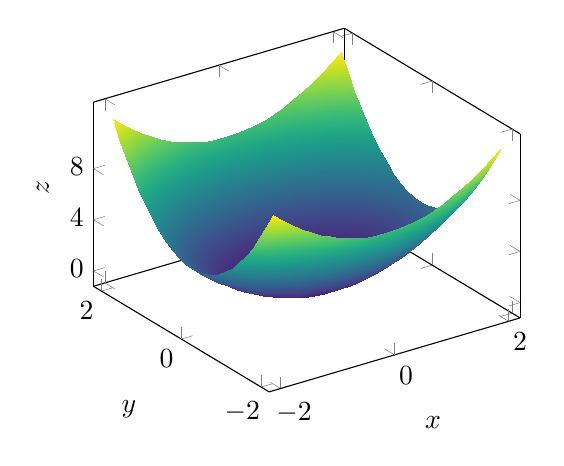
\begin{tikzpicture}
\begin{axis}[width=7cm,height=6.2cm,view={-35}{35},colormap/viridis,
  xlabel=$x$,ylabel=$y$,zlabel=$z$,xtick={-2,0,2},ytick={-2,0,2},ztick={0,4,8},
  xmin=-2.2,xmax=2.2,ymin=-2.2,ymax=2.2]
  \addplot3[surf,shader=interp,domain=-2:2,y domain=-2:2,samples=25]{x^2+2*y^2};
\end{axis}
\end{tikzpicture}\hfill
\begin{tikzpicture}[scale=0.95]
  \draw[-{Stealth[length=2mm]},gray] (-2.6,0) -- (2.7,0) node[right] {$x$};
  \draw[-{Stealth[length=2mm]},gray] (0,-2.0) -- (0,2.1) node[above] {$y$};
  \foreach \c/\col in {0.5/20,1/35,2/50,3/65,4/80}
    \draw[thick,MLdef!\col!PlotGreen] (0,0) ellipse ({sqrt(\c)} and {sqrt(\c/2)});
  \foreach \c in {1,2,4}
    \node[font=\scriptsize,fill=white,inner sep=1pt] at ({sqrt(\c)},0.25) {$\c$};
\end{tikzpicture}
\caption{Two pictures of $f(x, y) = x^2 + 2y^2$. Left: its graph, a bowl-shaped
  surface. Right: its contour plot, the ellipses $x^2 + 2y^2 = c$ for
  $c = 0.5, 1, 2, 3, 4$ (some labelled). The contours are closer together in the
  $y$-direction, where the bowl is steeper.}
\label{fig:surface-contour}
\end{figure}

\begin{mlnote}[Loss landscapes]
The graph of the loss as a function of the parameters is called the
\emph{loss landscape}. For a model with two parameters we can draw it, and
training looks like a ball rolling down into a valley. For a real network the
landscape lives in millions of dimensions, but the intuition from two
dimensions (valleys, ridges, saddles, flat plateaus) remains the main way
practitioners think about training.
\end{mlnote}

\sectionexercises

\begin{exercise}
Let $f(x, y) = x^2 - y + 3$. Evaluate $f(2, 1)$, and describe the level curve
$f(x, y) = 3$.
\end{exercise}
\begin{solution}
$f(2,1) = 4 - 1 + 3 = 6$. The level curve $x^2 - y + 3 = 3$ is $y = x^2$, a
parabola.
\end{solution}

\begin{exercise}
Describe the contour lines of $f(x, y) = x + 2y$ and of
$g(x, y) = x^2 + y^2$.
\end{exercise}
\begin{solution}
$x + 2y = c$ are parallel straight lines with slope $-\tfrac12$ (a tilted plane
has straight, evenly spaced contours). $x^2 + y^2 = c$ are circles centred at
the origin with radius $\sqrt c$ (a round bowl).
\end{solution}

\begin{exercise}
For the two data points $(x, y) = (1, 2)$ and $(2, 4)$, the mean squared error
of the model $\hat y = wx + b$ is
$L(w, b) = \frac12\left[(2 - w - b)^2 + (4 - 2w - b)^2\right]$. Evaluate
$L(2, 0)$ and $L(1, 1)$. Which parameters fit better?
\end{exercise}
\begin{solution}
$L(2, 0) = \tfrac12[0 + 0] = 0$: a perfect fit ($y = 2x$). $L(1, 1) =
\tfrac12[0 + (4 - 3)^2] = 0.5$. The parameters $(2, 0)$ fit better.
\end{solution}

%----------------------------------------------------------------------
\section{Partial derivatives}\label{sec:partial-derivatives}
%----------------------------------------------------------------------

The simplest way to measure how a function of several variables changes is to
change \emph{one} variable at a time, keeping all the others fixed.

\begin{definition}[Partial derivative]\label{def:partial-derivative}
The \term{partial derivative} of $f(x, y)$ with respect to $x$ is
\[
  \pderiv{f}{x}(x, y) = \lim_{h\to0}\frac{f(x + h, y) - f(x, y)}{h},
\]
the derivative of $f$ with respect to $x$ when $y$ is held constant. The
partial derivative $\pderiv{f}{y}$ is defined in the same way, holding $x$
constant. For a function of $n$ variables there is one partial derivative
$\pderiv{f}{x_i}$ for each variable.
\end{definition}

\begin{notation}
The curly $\partial$ (``partial'' or ``del'') signals that other variables are
being held fixed. Common alternatives are $f_x$, $\partial_x f$ and
$\partial f/\partial x$. So $\pderiv{f}{x}$ is read ``partial $f$ by partial
$x$'' or ``the partial derivative of $f$ with respect to $x$''.
\end{notation}

\begin{picturethis}
Slice the surface $z = f(x, y)$ with the vertical plane $y = y_0$. The cut is a
curve, the graph of the one-variable function $x \mapsto f(x, y_0)$. The partial
derivative $\pderiv{f}{x}(x_0, y_0)$ is the slope of that curve at $x_0$: the
steepness of the surface if you walk in the $x$-direction
(\cref{fig:partial-slice}).
\end{picturethis}

\begin{figure}[htbp]
\centering
\begin{tikzpicture}
\begin{axis}[width=8.5cm,height=7cm,view={-30}{28},colormap/viridis,
  xlabel=$x$,ylabel=$y$,zlabel=$z$,xmin=-1.6,xmax=1.6,ymin=-1.6,ymax=1.6,
  zmin=0,zmax=4.5,xtick={-1,0,1},ytick={-1,0,1},ztick={0,2,4}]
  \addplot3[surf,shader=interp,opacity=0.7,domain=-1.5:1.5,y domain=-1.5:1.5,samples=25]{4-x^2-y^2};
  \addplot3[PlotRed,line width=1.6pt,samples=40,samples y=1,domain=-1.5:1.5] (x,0.5,{3.75-x^2});
  \addplot3[black,thick,samples=2,samples y=1,domain=-0.4:1.4] (x,0.5,{3.5-(x-0.5)});
  \addplot3[only marks,mark=*,mark size=2.2pt] coordinates {(0.5,0.5,3.5)};
\end{axis}
\end{tikzpicture}
\caption{The surface $z = 4 - x^2 - y^2$ cut by the plane $y = 0.5$ (red
  curve). The partial derivative $\pderiv{f}{x}(0.5, 0.5) = -2(0.5) = -1$ is the
  slope of the black tangent line to the red curve.}
\label{fig:partial-slice}
\end{figure}

\subsection{Computing partial derivatives}

There is nothing new to learn: treat every other variable as if it were a
number, and use the rules of \cref{ch:calculus}.

\begin{example}[Partial derivatives]\label{ex:partials}
Compute the partial derivatives of (a) $f(x, y) = x^2y + 3y^3$;
(b) $g(x, y) = e^{xy}$; (c) $h(x, y) = \ln(x^2 + y^2)$.

\sol (a) With $y$ constant, $x^2y$ behaves like ``constant times $x^2$'' and
$3y^3$ is a constant: $\pderiv{f}{x} = 2xy$. With $x$ constant:
$\pderiv{f}{y} = x^2 + 9y^2$.

(b) By the chain rule, $\pderiv{g}{x} = e^{xy}\cdot y = y\,e^{xy}$ and
$\pderiv{g}{y} = x\,e^{xy}$.

(c) $\pderiv{h}{x} = \frac{2x}{x^2 + y^2}$ and $\pderiv{h}{y} =
\frac{2y}{x^2 + y^2}$.
\end{example}

\subsection{Higher-order partial derivatives}

Partial derivatives are themselves functions of $x$ and $y$, so we can
differentiate them again. There are four second-order partial derivatives of
$f(x,y)$:
\[
  \frac{\partial^2 f}{\partial x^2},\qquad
  \frac{\partial^2 f}{\partial y^2},\qquad
  \frac{\partial^2 f}{\partial y\,\partial x}
    = \frac{\partial}{\partial y}\left(\pderiv{f}{x}\right),\qquad
  \frac{\partial^2 f}{\partial x\,\partial y}
    = \frac{\partial}{\partial x}\left(\pderiv{f}{y}\right).
\]
For $f = x^2y + 3y^3$: $f_{xx} = 2y$, $f_{yy} = 18y$, and both mixed partials
equal $2x$. That the mixed partials agree is no accident.

\begin{theorem}[Symmetry of mixed partials]\label{thm:clairaut}
If the second partial derivatives of $f$ are continuous, then
$\frac{\partial^2 f}{\partial x\,\partial y} = \frac{\partial^2 f}{\partial
y\,\partial x}$: the order of differentiation does not matter.
\end{theorem}

\begin{mlnote}[One weight at a time]
For a model with weights $w_1, \dots, w_n$, the partial derivative
$\pderiv{L}{w_i}$ answers: ``if I change only $w_i$ a tiny bit, how fast does the
loss change?'' For example, for a single data point $(x, y)$ and the model
$\hat y = wx + b$ with squared error $L(w, b) = (y - wx - b)^2$, the chain rule
gives
\[
  \pderiv{L}{w} = -2x(y - wx - b), \qquad \pderiv{L}{b} = -2(y - wx - b).
\]
Both are proportional to the error $y - \hat y$: parameters are adjusted more
when the prediction is worse, and the weight $w$ more when the input $x$ is
larger.
\end{mlnote}

\sectionexercises

\begin{exercise}
Find $\pderiv{f}{x}$ and $\pderiv{f}{y}$ for $f(x, y) = 3x^2y - 2xy^3 + 5$.
\end{exercise}
\begin{solution}
$\pderiv{f}{x} = 6xy - 2y^3$ and $\pderiv{f}{y} = 3x^2 - 6xy^2$.
\end{solution}

\begin{exercise}
Find the partial derivatives of $f(x, y) = x\,e^y + \ln x$.
\end{exercise}
\begin{solution}
$\pderiv{f}{x} = e^y + \tfrac1x$ and $\pderiv{f}{y} = x\,e^y$.
\end{solution}

\begin{exercise}
For $f(x, y) = \sin(xy)$, compute $f_x$, $f_y$, and both mixed second partial
derivatives, and check that they agree.
\end{exercise}
\begin{solution}
$f_x = y\cos(xy)$ and $f_y = x\cos(xy)$. Then
$\tfrac{\partial}{\partial y}(y\cos(xy)) = \cos(xy) - xy\sin(xy)$ (product
rule), and $\tfrac{\partial}{\partial x}(x\cos(xy)) = \cos(xy) - xy\sin(xy)$.
They agree.
\end{solution}

\begin{exercise}
For the single-point loss $L(w, b) = (y - wx - b)^2$ with $x = 2$ and $y = 7$,
compute both partial derivatives at $w = 1$, $b = 1$.
\end{exercise}
\begin{solution}
The error is $y - wx - b = 7 - 2 - 1 = 4$. So $\pderiv{L}{w} = -2\cdot2\cdot4 =
-16$ and $\pderiv{L}{b} = -2\cdot4 = -8$. Both are negative: increasing either
parameter reduces the loss, and $w$ has the larger effect.
\end{solution}

%----------------------------------------------------------------------
\section{The gradient}\label{sec:gradient}
%----------------------------------------------------------------------

\begin{definition}[Gradient]\label{def:gradient}
The \term{gradient} of $f\colon\R^n\to\R$ at $\vx$ is the vector of all its
partial derivatives:
\[
  \keyeq{\nabla f(\vx) = \begin{pmatrix} \pderiv{f}{x_1}(\vx)\\ \vdots\\
  \pderiv{f}{x_n}(\vx)\end{pmatrix}}
\]
The symbol $\nabla$ is called ``nabla'' or ``del'', and $\nabla f$ is read
``grad $f$''. When it is important to say which variables we differentiate
with respect to, we write, for example, $\nabla_{\vw}L$.
\end{definition}

The gradient packs $n$ numbers into one vector that lives in the same space as
the input $\vx$. For $f(x, y) = x^2 + y^2$, $\nabla f = (2x, 2y)$; at the point
$(1, 2)$ the gradient is $(2, 4)$.

\begin{example}[Gradients of common functions of vectors]\label{ex:vector-gradients}
For $\vx \in \R^n$:
\begin{enumerate}
  \item $f(\vx) = \va^\top\vx = a_1x_1 + \dots + a_nx_n$: each partial derivative
    is $\pderiv{f}{x_i} = a_i$, so $\nabla f = \va$. (The analogue of
    $\frac{\dd}{\dd x}ax = a$.)
  \item $f(\vx) = \norm{\vx}^2 = x_1^2 + \dots + x_n^2$: $\pderiv{f}{x_i} = 2x_i$,
    so $\nabla f = 2\vx$. (The analogue of $\frac{\dd}{\dd x}x^2 = 2x$.)
  \item $f(\vx) = \norm{\vx - \va}^2$: by the chain rule, $\nabla f = 2(\vx - \va)$.
\end{enumerate}
\end{example}

\subsection{The geometry of the gradient}

\begin{theorem}[The gradient points uphill]\label{thm:gradient-geometry}
At any point where $\nabla f \neq \vzero$:
\begin{enumerate}
  \item $\nabla f$ points in the direction in which $f$ increases fastest
    (\emph{steepest ascent}), and $-\nabla f$ in the direction of steepest
    descent;
  \item the length $\norm{\nabla f}$ is the rate of increase in that direction;
  \item $\nabla f$ is perpendicular to the level curve (contour) through the
    point.
\end{enumerate}
\end{theorem}

We prove this in \cref{sec:directional-derivatives}. \Cref{fig:gradient-field}
shows the picture: gradient arrows cross the contour lines at right angles,
pointing uphill, and are longest where the contours are most crowded.

\begin{figure}[htbp]
\centering
\begin{tikzpicture}[scale=1.15]
  \draw[-{Stealth[length=2mm]},gray] (-3,0) -- (3.1,0) node[right] {$x$};
  \draw[-{Stealth[length=2mm]},gray] (0,-1.9) -- (0,2.0) node[above] {$y$};
  \foreach \c in {0.75,3,6.75}
    \draw[thick,MLdef] (0,0) ellipse ({sqrt(\c)} and {sqrt(\c/3)});
  \foreach \p/\g in {{1.732,0}/{3.464,0},{0,1}/{0,6},{1.5,0.5}/{3,3},{-1.5,0.5}/{-3,3},
                     {1,-0.8165}/{2,-4.899},{-1.732,0}/{-3.464,0},{-1,-0.8165}/{-2,-4.899}}
    \draw[-{Stealth[length=2mm]},thick,PlotRed] (\p) -- ++($0.15*(\g)$);
  \draw[-{Stealth[length=2mm]},very thick,PlotGreen!70!black] (1.5,0.5) -- ++(-0.45,-0.45)
    node[below left=-1pt,font=\small] {$-\nabla f$};
  \foreach \p in {{1.732,0},{0,1},{1.5,0.5},{-1.5,0.5},{1,-0.8165},{-1.732,0},{-1,-0.8165}}
    \fill (\p) circle (1.2pt);
\end{tikzpicture}
\caption{Contours of $f(x, y) = x^2 + 3y^2$ (blue) and gradient vectors
  $\nabla f = (2x, 6y)$ at points of the middle contour (red, scaled down). Each
  gradient is perpendicular to the contour and points uphill; the green arrow
  is the direction of steepest descent.}
\label{fig:gradient-field}
\end{figure}

At a minimum or maximum of a differentiable function, there is no uphill
direction, so the gradient is zero. Points with $\nabla f = \vzero$ are called
\emph{critical points}, as in one variable.

\subsection{Linear approximation and the tangent plane}

The one-variable approximation $f(a + h) \approx f(a) + f'(a)h$ becomes
\[
  \keyeq{f(\vx + \vh) \approx f(\vx) + \nabla f(\vx)^\top\vh}
\]
for a small vector $\vh$: each variable contributes its partial derivative
times its own change, and the contributions add up. For two variables, the graph
of the right-hand side is the \emph{tangent plane} to the surface. This formula
is the reason the gradient governs optimisation.

\begin{example}[The gradient of a regression loss]\label{ex:regression-gradient}
For the data $(1, 2)$, $(2, 3)$, $(3, 5)$ and the model $\hat y = wx + b$, the
mean squared error is $L(w, b) = \frac13\sum_{i=1}^3(y_i - wx_i - b)^2$. Compute
$\nabla L$ at $(w, b) = (0, 0)$ and find where $\nabla L = \vzero$.

\sol Write $r_i = y_i - wx_i - b$ for the residuals. By the chain rule,
\[
  \pderiv{L}{w} = -\frac23\sum_i x_ir_i, \qquad
  \pderiv{L}{b} = -\frac23\sum_i r_i .
\]
At $(0, 0)$ the residuals are just $(2, 3, 5)$, so
$\pderiv{L}{w} = -\frac23(2 + 6 + 15) \approx -15.3$ and
$\pderiv{L}{b} = -\frac23(10) \approx -6.67$. The gradient
$(-15.3, -6.67)$ points towards smaller $w$ and $b$; the loss \emph{decreases}
fastest in the opposite direction, so training would increase both
parameters, and $w$ faster than $b$.

Setting both partial derivatives to zero gives $\sum_i x_ir_i = 0$ and
$\sum_i r_i = 0$: the residuals must be orthogonal to the column of inputs and
to the column of ones. These are exactly the normal equations of
\cref{sec:projections}, with solution $w = 1.5$, $b = \frac13$. Calculus and
geometry give the same answer.
\end{example}

\sectionexercises

\begin{exercise}
Compute the gradient of $f(x, y) = x^2y + y^3$ at the point $(1, 2)$.
\end{exercise}
\begin{solution}
$\nabla f = (2xy, x^2 + 3y^2)$, so $\nabla f(1, 2) = (4, 1 + 12) = (4, 13)$.
\end{solution}

\begin{exercise}
Find the critical point of $f(x, y) = x^2 + y^2 - 2x + 4y$.
\end{exercise}
\begin{solution}
$\nabla f = (2x - 2, 2y + 4) = \vzero$ gives $(x, y) = (1, -2)$. (Completing the
square, $f = (x - 1)^2 + (y + 2)^2 - 5$, so this is the minimum, with value
$-5$.)
\end{solution}

\begin{exercise}
Use the linear approximation at $(1, 1)$ to estimate $f(1.1, 0.9)$ for
$f(x, y) = x^2 + y^2$, and compare with the exact value.
\end{exercise}
\begin{solution}
$f(1, 1) = 2$ and $\nabla f(1,1) = (2, 2)$, so
$f(1.1, 0.9) \approx 2 + (2, 2)\cdot(0.1, -0.1) = 2$. The exact value is
$1.21 + 0.81 = 2.02$; the small error comes from the curvature.
\end{solution}

\begin{exercise}
For the data $(1, 1)$ and $(2, 3)$ and the model $\hat y = wx + b$ with mean
squared error, compute $\nabla L$ at $(w, b) = (1, 0)$.
\end{exercise}
\begin{solution}
Residuals $r_i = y_i - wx_i - b$: $1 - 1 = 0$ and $3 - 2 = 1$. With $n = 2$:
$\pderiv{L}{w} = -\tfrac22(1\cdot0 + 2\cdot1) = -2$ and
$\pderiv{L}{b} = -\tfrac22(0 + 1) = -1$. So $\nabla L = (-2, -1)$.
\end{solution}

%----------------------------------------------------------------------
\section{Directional derivatives}\label{sec:directional-derivatives}
%----------------------------------------------------------------------

Partial derivatives measure the rate of change along the coordinate axes. What
about other directions?

\begin{definition}[Directional derivative]\label{def:directional-derivative}
The \term{directional derivative} of $f$ at $\vx$ in the direction of a unit
vector $\vu$ is
\[
  D_{\vu}f(\vx) = \lim_{h\to0}\frac{f(\vx + h\vu) - f(\vx)}{h},
\]
the rate of change of $f$ as we move from $\vx$ in the direction $\vu$.
\end{definition}

By the linear approximation, $f(\vx + h\vu) \approx f(\vx) + h\,\nabla
f(\vx)^\top\vu$, so

\begin{theorem}[Directional derivatives from the gradient]\label{thm:directional}
\[
  D_{\vu}f(\vx) = \nabla f(\vx)\cdot\vu .
\]
\end{theorem}

Now the geometry of the gradient follows from the geometry of the dot product.
By \cref{thm:dot-geometric}, $\nabla f\cdot\vu = \norm{\nabla f}\cos\theta$, where
$\theta$ is the angle between $\vu$ and the gradient. This is largest
(namely $\norm{\nabla f}$) when $\theta = 0$, i.e.\ when $\vu$ points along
$\nabla f$; smallest (namely $-\norm{\nabla f}$) when $\vu$ points along
$-\nabla f$; and zero when $\vu$ is perpendicular to $\nabla f$. Moving along a
contour line does not change $f$, so the direction of the contour has zero
directional derivative, which means it is perpendicular to the gradient. This
proves \cref{thm:gradient-geometry}.

\begin{example}[Directional derivatives]
Let $f(x, y) = x^2 + 3y^2$ and $\vx = (1, 1)$, so $\nabla f = (2, 6)$.
\begin{itemize}
  \item In the direction $\vu = (1, 0)$: $D_{\vu}f = 2$ (this is just
    $\pderiv{f}{x}$).
  \item In the direction $\vu = (0.6, 0.8)$: $D_{\vu}f = 1.2 + 4.8 = 6$.
  \item The steepest direction is $\frac{(2, 6)}{\norm{(2,6)}}$, with rate
    $\norm{(2, 6)} = \sqrt{40} \approx 6.32$; no direction gives a faster
    increase.
\end{itemize}
\end{example}

\begin{mlnote}[Steepest descent]
To decrease a loss as quickly as possible from the current parameters, move in
the direction $-\nabla L$. This is the idea of \emph{gradient descent}:
repeatedly replace the parameters $\vtheta$ by $\vtheta - \eta\nabla L(\vtheta)$
for a small step size $\eta$ (\cref{ch:optimization}). The steepest direction
is only steepest \emph{locally}, which is why the steps must be small and
repeated many times.
\end{mlnote}

\sectionexercises

\begin{exercise}
For $f(x, y) = x^2 + 3y^2$ at $(1, 1)$, compute the directional derivative in
the direction of $(1, 1)$. (Remember to normalise.)
\end{exercise}
\begin{solution}
$\vu = \tfrac{1}{\sqrt2}(1, 1)$ and $\nabla f(1,1) = (2, 6)$, so
$D_{\vu}f = \tfrac{2 + 6}{\sqrt2} = 4\sqrt2 \approx 5.66$.
\end{solution}

\begin{exercise}
For $f(x, y) = xy$ at the point $(2, 3)$: in which direction does $f$ increase
fastest, and at what rate? In which directions does $f$ not change at all?
\end{exercise}
\begin{solution}
$\nabla f = (y, x) = (3, 2)$. Fastest increase in the direction
$\tfrac{1}{\sqrt{13}}(3, 2)$, at rate $\sqrt{13} \approx 3.61$. No change in the
directions perpendicular to $(3, 2)$, i.e.\ $\pm\tfrac{1}{\sqrt{13}}(2, -3)$.
\end{solution}

\begin{exercise}
What is the directional derivative of $f$ at a minimum, in any direction?
\end{exercise}
\begin{solution}
At an interior minimum of a differentiable function, $\nabla f = \vzero$, so
$D_{\vu}f = \vzero\cdot\vu = 0$ in every direction.
\end{solution}

%----------------------------------------------------------------------
\section{The chain rule for several variables}\label{sec:multivariable-chain-rule}
%----------------------------------------------------------------------

\subsection{One input, several paths}

Suppose $z = f(x, y)$ and both $x$ and $y$ depend on a single variable $t$.
When $t$ changes a little, it changes $x$, which changes $z$; and it changes
$y$, which also changes $z$. The total effect is the sum of the two effects.

\begin{theorem}[Chain rule, two intermediate variables]\label{thm:chain-two}
If $z = f(x, y)$ with $x = x(t)$ and $y = y(t)$, then
\[
  \deriv{z}{t} = \pderiv{z}{x}\deriv{x}{t} + \pderiv{z}{y}\deriv{y}{t}.
\]
\end{theorem}

\begin{figure}[htbp]
\centering
\begin{tikzpicture}[>={Stealth[length=2.2mm]},
  nd/.style={circle,draw,thick,minimum size=8mm,fill=MLdef!10}]
  \node[nd] (z) at (0,3.2) {$z$};
  \node[nd] (x) at (-2.3,1.6) {$x$};
  \node[nd] (y) at (2.3,1.6) {$y$};
  \node[nd] (t) at (0,0) {$t$};
  \draw[->,thick] (t) -- node[below left] {$\dd x/\dd t$} (x);
  \draw[->,thick] (t) -- node[below right] {$\dd y/\dd t$} (y);
  \draw[->,thick] (x) -- node[above left] {$\partial z/\partial x$} (z);
  \draw[->,thick] (y) -- node[above right] {$\partial z/\partial y$} (z);
\end{tikzpicture}
\caption{Dependency diagram for $z = f(x(t), y(t))$. The derivative
  $\deriv{z}{t}$ is the sum, over the two paths from $t$ to $z$, of the products
  of the derivatives along each path.}
\label{fig:chain-tree}
\end{figure}

\begin{example}[Chain rule along two paths]
Let $z = x^2y$ with $x = \cos t$ and $y = \sin t$. Find $\deriv{z}{t}$ at $t = 0$.

\sol $\pderiv{z}{x} = 2xy$, $\pderiv{z}{y} = x^2$, $\deriv{x}{t} = -\sin t$ and
$\deriv{y}{t} = \cos t$. At $t = 0$: $x = 1$, $y = 0$, so
$\deriv{z}{t} = 2\cdot1\cdot0\cdot0 + 1\cdot1 = 1$. (Check:
$z = \cos^2t\,\sin t$, whose derivative at $0$ is $-2\cos t\sin^2t + \cos^3t
= 1$.)
\end{example}

\subsection{The general rule: sum over paths}

The same principle works for any number of variables and any number of
layers.

\begin{theorem}[General chain rule]\label{thm:chain-general}
If $z$ depends on intermediate variables $u_1, \dots, u_m$, each of which
depends on $x$, then
\[
  \keyeq{\pderiv{z}{x} = \sum_{k=1}^{m}\pderiv{z}{u_k}\,\pderiv{u_k}{x}}
\]
More generally, in any network of dependencies, $\pderiv{z}{x}$ is the sum, over
all paths from $x$ to $z$, of the product of the local derivatives along the
path.
\end{theorem}

\subsection{Computation graphs}

Any formula can be broken into elementary steps and drawn as a
\term{computation graph}: each node is an intermediate value, and arrows show
which values are used to compute which. Derivatives can then be computed
mechanically, one node at a time.

\begin{example}[Gradients on a computation graph]\label{ex:computation-graph}
Let $f(x, y) = (x + y)(y + 1)$. Introduce $a = x + y$ and $b = y + 1$, so that
$f = ab$. Compute all partial derivatives at $x = 2$, $y = 3$.

\sol \emph{Forward pass} (compute values): $a = 5$, $b = 4$, $f = 20$.

\emph{Backward pass} (compute derivatives, from the output back to the
inputs). The local derivatives of $f = ab$ are $\pderiv{f}{a} = b = 4$ and
$\pderiv{f}{b} = a = 5$. Next, $x$ influences $f$ only through $a$, with
$\pderiv{a}{x} = 1$, so $\pderiv{f}{x} = 4\cdot1 = 4$. But $y$ influences $f$
along two paths, through $a$ and through $b$, so we add:
\[
  \pderiv{f}{y} = \pderiv{f}{a}\pderiv{a}{y} + \pderiv{f}{b}\pderiv{b}{y}
  = 4\cdot1 + 5\cdot1 = 9 .
\]
\emph{Check} by expanding: $f = xy + x + y^2 + y$, so $f_x = y + 1 = 4$ and
$f_y = x + 2y + 1 = 9$. \checkmark
\end{example}

\begin{figure}[htbp]
\centering
\begin{tikzpicture}[>={Stealth[length=2.5mm]},
  var/.style={circle,draw,thick,minimum size=9mm,fill=MLdef!10},
  op/.style={rounded corners,draw,thick,minimum size=8mm,fill=MLexample!12},
  fwd/.style={font=\small,text=PlotBlue},
  bwd/.style={font=\small,text=PlotRed}]
  \node[var] (x) at (0,1.8) {$x$};
  \node[var] (y) at (0,-0.4) {$y$};
  \node[op] (a) at (3.2,1.8) {$a = x + y$};
  \node[op] (b) at (3.2,-0.4) {$b = y + 1$};
  \node[op] (f) at (6.6,0.7) {$f = ab$};
  \draw[->,thick] (x) -- (a);
  \draw[->,thick] (y) -- (a);
  \draw[->,thick] (y) -- (b);
  \draw[->,thick] (a) -- (f);
  \draw[->,thick] (b) -- (f);
  \node[fwd,above=1pt] at (x.north) {$2$};
  \node[fwd,below=1pt] at (y.south) {$3$};
  \node[fwd,above=1pt] at (a.north) {$5$};
  \node[fwd,below=1pt] at (b.south) {$4$};
  \node[fwd,above=1pt] at (f.north) {$20$};
  \node[bwd,left=2pt] at (x.west) {$\pderiv{f}{x} = 4$};
  \node[bwd,left=2pt] at (y.west) {$\pderiv{f}{y} = 4 + 5 = 9$};
  \node[bwd] at (5.0,1.75) {$\pderiv{f}{a} = 4$};
  \node[bwd] at (5.0,-0.35) {$\pderiv{f}{b} = 5$};
\end{tikzpicture}
\caption{The computation graph of $f = (x + y)(y + 1)$ at $x = 2$, $y = 3$.
  Forward values are in blue; derivatives of the output, computed backwards,
  are in red. The two paths from $y$ to $f$ contribute $4$ and $5$.}
\label{fig:computation-graph}
\end{figure}

\begin{mlnote}[Backpropagation is the chain rule on a computation graph]
A neural network and its loss form one large computation graph, with the
weights as inputs and the loss as output. \emph{Backpropagation} computes
$\pderiv{L}{w}$ for every weight by exactly the procedure of
\cref{ex:computation-graph}: one forward pass to compute all intermediate
values, then one backward pass that multiplies local derivatives and adds them
up wherever paths merge. Its great virtue is efficiency: the derivatives of all
the weights are obtained for roughly the cost of two evaluations of the
network, because the products along shared parts of the paths are computed once
and reused. We will carry this out in detail in \cref{ch:dl}.
\end{mlnote}

\sectionexercises

\begin{exercise}
Let $z = x^2 + y^2$ with $x = 2t$ and $y = t^2$. Find $\deriv{z}{t}$ with the
chain rule, and check by substituting first.
\end{exercise}
\begin{solution}
$\deriv{z}{t} = 2x\cdot2 + 2y\cdot2t = 8t + 4t^3$ (using $x = 2t$, $y = t^2$).
Check: $z = 4t^2 + t^4$, so $\deriv{z}{t} = 8t + 4t^3$.
\end{solution}

\begin{exercise}
Let $f(x, y) = xy$ with $x = 3t + 1$ and $y = t^2$. Find $\deriv{f}{t}$ at
$t = 1$.
\end{exercise}
\begin{solution}
At $t = 1$: $x = 4$, $y = 1$. $\deriv{f}{t} = y\cdot3 + x\cdot2t = 3 + 8 = 11$.
(Check: $f = 3t^3 + t^2$, so $f' = 9t^2 + 2t = 11$ at $t = 1$.)
\end{solution}

\begin{exercise}
Draw the computation graph of $f(x, y, z) = xy + z$ (with $q = xy$) and compute
the forward value and all three partial derivatives at $x = -2$, $y = 5$,
$z = -4$.
\end{exercise}
\begin{solution}
Forward: $q = -10$, $f = q + z = -14$. Backward: $\pderiv{f}{q} = 1$ and
$\pderiv{f}{z} = 1$; then $\pderiv{f}{x} = \pderiv{f}{q}\cdot y = 5$ and
$\pderiv{f}{y} = \pderiv{f}{q}\cdot x = -2$.
\end{solution}

\begin{exercise}
A neuron computes $\hat y = \sigma(w_1x_1 + w_2x_2 + b)$ with squared error
$L = (\hat y - y)^2$. Use the chain rule to write $\pderiv{L}{w_1}$,
$\pderiv{L}{w_2}$ and $\pderiv{L}{b}$, and evaluate them for $\vx = (1, 2)$,
$\vw = (0.5, -0.5)$, $b = 0$, $y = 1$.
\end{exercise}
\begin{solution}
With $z = w_1x_1 + w_2x_2 + b$: $\pderiv{L}{w_i} = 2(\hat y - y)\,\sigma'(z)\,x_i$
and $\pderiv{L}{b} = 2(\hat y - y)\,\sigma'(z)$. Here $z = 0.5 - 1 = -0.5$,
$\hat y = \sigma(-0.5) \approx 0.378$ and $\sigma'(z) = \hat y(1 - \hat y)
\approx 0.235$. So $2(\hat y - y)\sigma'(z) \approx 2(-0.622)(0.235) \approx
-0.293$, giving $\pderiv{L}{w_1} \approx -0.293$, $\pderiv{L}{w_2} \approx
-0.585$ and $\pderiv{L}{b} \approx -0.293$.
\end{solution}

%----------------------------------------------------------------------
\section{Vector-valued functions and the Jacobian}\label{sec:jacobian}
%----------------------------------------------------------------------

A neural network layer takes a vector and returns a vector. Its derivative
must describe how \emph{each} output depends on \emph{each} input, which calls for
a matrix.

\begin{definition}[Jacobian matrix]\label{def:jacobian}
Let $\vf\colon\R^n\to\R^m$ have component functions $f_1, \dots, f_m$. Its
\term{Jacobian matrix} at $\vx$ is the $m\times n$ matrix of all first partial
derivatives:
\[
  \mat{J}_{\vf}(\vx) = \begin{pmatrix}
    \pderiv{f_1}{x_1} & \cdots & \pderiv{f_1}{x_n}\\
    \vdots & \ddots & \vdots\\
    \pderiv{f_m}{x_1} & \cdots & \pderiv{f_m}{x_n}
  \end{pmatrix},
  \qquad (\mat{J}_{\vf})_{ij} = \pderiv{f_i}{x_j}.
\]
Row $i$ is the gradient of $f_i$, written as a row.
\end{definition}

\begin{example}[Jacobians]\label{ex:jacobians}
(a) For $\vf(x, y) = (x^2y,\ 5x + \sin y)$:
$\mat{J} = \left(\begin{smallmatrix} 2xy & x^2\\ 5 & \cos y\end{smallmatrix}\right)$.

(b) For a linear map $\vf(\vx) = \mA\vx + \vb$, each $f_i = \sum_j a_{ij}x_j + b_i$
has $\pderiv{f_i}{x_j} = a_{ij}$, so $\mat{J} = \mA$: the derivative of a linear
map is the matrix itself.

(c) For an activation applied to each component, $\vf(\vz) = (\sigma(z_1),
\dots, \sigma(z_n))$, output $i$ depends only on input $i$, so the Jacobian is
diagonal: $\mat{J} = \diag\bigl(\sigma'(z_1), \dots, \sigma'(z_n)\bigr)$.
\end{example}

The Jacobian gives the best linear approximation of $\vf$ near $\vx$:
\[
  \vf(\vx + \vh) \approx \vf(\vx) + \mat{J}_{\vf}(\vx)\,\vh .
\]
In the language of \cref{ch:linalg1}: zoomed in close enough, any smooth map
looks like a linear transformation, and its matrix is the Jacobian.

\begin{theorem}[Chain rule in matrix form]\label{thm:chain-matrix}
If $\vg\colon\R^n\to\R^m$ and $\vf\colon\R^m\to\R^p$ are differentiable, then
\[
  \keyeq{\mat{J}_{\vf\circ\vg}(\vx) = \mat{J}_{\vf}\bigl(\vg(\vx)\bigr)\,\mat{J}_{\vg}(\vx)}
\]
The Jacobian of a composition is the product of the Jacobians.
\end{theorem}

This is the ``sum over paths'' rule written with matrices: entry $(i, j)$ of
the product is $\sum_k \pderiv{f_i}{g_k}\pderiv{g_k}{x_j}$. It also matches
\cref{sec:matrix-multiplication}: composing linear maps multiplies their
matrices, and a composition of smooth maps is, locally, a composition of their
linear approximations.

\begin{example}[The Jacobian of a layer]\label{ex:layer-jacobian}
A layer computes $\vh = \ReLU(\mW\vx + \vb)$. Writing $\vz = \mW\vx + \vb$, the
chain rule gives
\[
  \pderiv{\vh}{\vx} = \diag\bigl(\ReLU'(z_1), \dots, \ReLU'(z_m)\bigr)\,\mW ,
\]
i.e.\ $\mW$ with the rows of the ``inactive'' neurons (those with $z_i < 0$) set to
zero. For instance, with the layer of \cref{sec:matrix-vector}, where
$\vz = (5.5, -2)$, the second neuron is inactive and the Jacobian is
$\left(\begin{smallmatrix} 1 & -1 & 2\\ 0 & 0 & 0\end{smallmatrix}\right)$.
\end{example}

\begin{remark}[Jacobian determinants change areas]
For a map from $\R^2$ to $\R^2$, the determinant of the Jacobian is the local
area-scaling factor (\cref{sec:inverses}). For polar coordinates,
$(r, \theta)\mapsto(r\cos\theta, r\sin\theta)$, the Jacobian is
$\left(\begin{smallmatrix} \cos\theta & -r\sin\theta\\ \sin\theta &
r\cos\theta\end{smallmatrix}\right)$, with determinant
$r\cos^2\theta + r\sin^2\theta = r$: small rectangles in the $(r,\theta)$-plane
become patches of area $r$ times larger. We use this in
\cref{sec:double-integrals}.
\end{remark}

\sectionexercises

\begin{exercise}
Find the Jacobian of $\vf(x, y) = (xy,\ x + y,\ x^2)$. What is its size?
\end{exercise}
\begin{solution}
$\left(\begin{smallmatrix} y & x\\ 1 & 1\\ 2x & 0\end{smallmatrix}\right)$, a
$3\times2$ matrix (three outputs, two inputs).
\end{solution}

\begin{exercise}
What is the Jacobian of $\vf(\vx) = \mA\vx + \vb$ with
$\mA = \left(\begin{smallmatrix} 1 & 2\\ 3 & 4\end{smallmatrix}\right)$? Does it
depend on $\vx$ or $\vb$?
\end{exercise}
\begin{solution}
It is $\mA$ itself, the same at every point, and it does not depend on $\vb$
(a shift does not affect rates of change).
\end{solution}

\begin{exercise}
Compute the Jacobian of the function that applies $\tanh$ to each component,
$\vf(\vz) = (\tanh z_1, \tanh z_2)$, at the point $\vz = (0, 1)$.
\end{exercise}
\begin{solution}
Diagonal, with entries $1 - \tanh^2 z_i$: at $(0, 1)$ this is
$\diag(1, 1 - \tanh^2 1) \approx \diag(1, 0.42)$.
\end{solution}

%----------------------------------------------------------------------
\section{The Hessian and the classification of critical points}\label{sec:hessian}
%----------------------------------------------------------------------

\begin{definition}[Hessian matrix]\label{def:hessian}
The \term{Hessian matrix} of $f\colon\R^n\to\R$ at $\vx$ is the $n\times n$ matrix
of second partial derivatives:
\[
  \mH(\vx) = \begin{pmatrix}
    \frac{\partial^2 f}{\partial x_1^2} & \cdots &
      \frac{\partial^2 f}{\partial x_1\,\partial x_n}\\
    \vdots & \ddots & \vdots\\
    \frac{\partial^2 f}{\partial x_n\,\partial x_1} & \cdots &
      \frac{\partial^2 f}{\partial x_n^2}
  \end{pmatrix}.
\]
By \cref{thm:clairaut} it is symmetric. It is the Jacobian of the gradient.
\end{definition}

\begin{example}[Hessians]\label{ex:hessians}
(a) $f = x^2 + 3y^2$: $\mH = \left(\begin{smallmatrix} 2 & 0\\ 0 &
6\end{smallmatrix}\right)$ (the same at every point).
(b) $f = x^2 - y^2$: $\mH = \left(\begin{smallmatrix} 2 & 0\\ 0 &
-2\end{smallmatrix}\right)$.
(c) $f = x^3 - 3x + y^2$: $\mH = \left(\begin{smallmatrix} 6x & 0\\ 0 &
2\end{smallmatrix}\right)$, which depends on the point.
(d) For a quadratic function $f(\vx) = \frac12\vx^\top\mA\vx + \vb^\top\vx + c$
with $\mA$ symmetric: $\nabla f = \mA\vx + \vb$ and $\mH = \mA$.
\end{example}

\subsection{Curvature in every direction}

The second derivative of $f$ along the line $\vx + t\vu$ (for a unit vector
$\vu$) is $\vu^\top\mH\vu$, a quadratic form. By \cref{sec:positive-definite},
its values are governed by the eigenvalues of $\mH$: the eigenvectors of the
Hessian are the directions of extreme curvature, and the eigenvalues are the
curvatures in those directions. A large eigenvalue means a steep, narrow
valley wall; a small one a gentle slope.

\subsection{The second derivative test in several variables}

\begin{theorem}[Second derivative test]\label{thm:second-derivative-test-multi}
Let $\nabla f(\vx^*) = \vzero$, with Hessian $\mH = \mH(\vx^*)$.
\begin{itemize}
  \item If $\mH$ is positive definite (all eigenvalues $> 0$), $\vx^*$ is a
    local minimum: the function curves upwards in every direction.
  \item If $\mH$ is negative definite (all eigenvalues $< 0$), $\vx^*$ is a
    local maximum.
  \item If $\mH$ has both positive and negative eigenvalues, $\vx^*$ is a
    \term{saddle point}: a minimum along some directions and a maximum along
    others.
  \item If $\mH$ is only semidefinite (some eigenvalue is $0$), the test is
    inconclusive.
\end{itemize}
For two variables: with $D = f_{xx}f_{yy} - f_{xy}^2 = \det\mH$, the point is a
minimum if $D > 0$ and $f_{xx} > 0$, a maximum if $D > 0$ and $f_{xx} < 0$, and a
saddle if $D < 0$.
\end{theorem}

The shapes are those of \cref{fig:quadratic-forms}: near a critical point,
$f(\vx^* + \vh) \approx f(\vx^*) + \frac12\vh^\top\mH\vh$, so the function looks
like the quadratic form of its Hessian.

\begin{example}[Classifying critical points]\label{ex:classify-2d}
Find and classify the critical points of $f(x, y) = x^3 - 3x + y^2$.

\sol $\nabla f = (3x^2 - 3,\ 2y) = \vzero$ gives $x = \pm1$, $y = 0$. The
Hessian is $\diag(6x, 2)$.
\begin{itemize}
  \item At $(1, 0)$: $\mH = \diag(6, 2)$, both eigenvalues positive: a local
    minimum, with $f(1, 0) = -2$.
  \item At $(-1, 0)$: $\mH = \diag(-6, 2)$, eigenvalues of opposite signs: a
    saddle point, with $f(-1,0) = 2$. Along the $x$-direction it is a maximum
    (of $x^3 - 3x$), along the $y$-direction a minimum (of $y^2$).
\end{itemize}
\end{example}

\begin{example}[A minimum with a non-diagonal Hessian]
Find the minimum of $f(x, y) = x^2 + xy + y^2 - 3x$.

\sol $\nabla f = (2x + y - 3,\ x + 2y) = \vzero$. The second equation gives
$x = -2y$; substituting, $-4y + y - 3 = 0$, so $y = -1$ and $x = 2$. The
Hessian $\left(\begin{smallmatrix} 2 & 1\\ 1 & 2\end{smallmatrix}\right)$ has
eigenvalues $3$ and $1$, so it is positive definite and $(2, -1)$ is a minimum,
with $f(2, -1) = 4 - 2 + 1 - 6 = -3$.
\end{example}

\begin{mlnote}[Saddles, curvature and the size of Hessians]
Three facts about Hessians shape how neural networks are trained.
\begin{itemize}
  \item \textbf{Saddle points are everywhere in high dimensions.} A critical
    point is a minimum only if \emph{all} eigenvalues of the Hessian are
    positive. With millions of parameters, it is far more common for at least
    a few to be negative, so most critical points of neural network losses are
    saddles, not minima. Gradient descent tends to escape them, because they
    have downhill directions.
  \item \textbf{Curvature limits the learning rate.} In a direction of
    curvature $\lambda$, a gradient step of size $\eta$ overshoots unless
    $\eta < 2/\lambda$ (\cref{ch:optimization}). A Hessian whose largest and
    smallest eigenvalues differ greatly (a large condition number) produces
    long, narrow valleys in which gradient descent zig-zags.
  \item \textbf{Hessians are too big to compute.} For a model with $10^9$
    parameters, the Hessian has $10^{18}$ entries. Deep learning therefore uses
    \emph{first-order} methods, which need only gradients, and approximates
    curvature information cheaply when it needs it (as the Adam optimiser
    does, \cref{ch:optimization}).
\end{itemize}
\end{mlnote}

\sectionexercises

\begin{exercise}
Compute the Hessian of $f(x, y) = x^3 + 2xy + y^2$.
\end{exercise}
\begin{solution}
$f_x = 3x^2 + 2y$, $f_y = 2x + 2y$; so $f_{xx} = 6x$, $f_{xy} = f_{yx} = 2$,
$f_{yy} = 2$, and $\mH = \left(\begin{smallmatrix} 6x & 2\\ 2 &
2\end{smallmatrix}\right)$.
\end{solution}

\begin{exercise}
Find and classify the critical point of $f(x, y) = x^2 + y^2 - 4x + 2y$.
\end{exercise}
\begin{solution}
$\nabla f = (2x - 4, 2y + 2) = \vzero$ at $(2, -1)$. $\mH = 2\mI$ is positive
definite, so it is a minimum, with value $4 + 1 - 8 - 2 = -5$.
\end{solution}

\begin{exercise}
Show that $(0, 0)$ is a saddle point of $f(x, y) = xy$.
\end{exercise}
\begin{solution}
$\nabla f = (y, x)$ vanishes at the origin. $\mH = \left(\begin{smallmatrix} 0 &
1\\ 1 & 0\end{smallmatrix}\right)$ has eigenvalues $1$ and $-1$ (with
eigenvectors $(1,1)$ and $(1,-1)$), so it is indefinite: $f$ increases along
the line $y = x$ (where $f = x^2$) and decreases along $y = -x$ (where
$f = -x^2$).
\end{solution}

\begin{exercise}
Find and classify all critical points of $f(x, y) = x^3 - 12x + y^3 - 3y$.
\end{exercise}
\begin{solution}
$\nabla f = (3x^2 - 12, 3y^2 - 3) = \vzero$ gives $x = \pm2$, $y = \pm1$: four
critical points. $\mH = \diag(6x, 6y)$. At $(2, 1)$: both positive, a minimum
($f = 8 - 24 + 1 - 3 = -18$). At $(-2, -1)$: both negative, a maximum
($f = 18$). At $(2, -1)$ and $(-2, 1)$: opposite signs, saddle points.
\end{solution}

\begin{exercise}
For $f(x, y) = x^4 + y^4$, show that the second derivative test is
inconclusive at the origin, but that the origin is a minimum.
\end{exercise}
\begin{solution}
$\nabla f = (4x^3, 4y^3)$ and $\mH = \diag(12x^2, 12y^2)$, which is the zero
matrix at the origin: inconclusive. But $f \ge 0 = f(0, 0)$ everywhere, so the
origin is a (global) minimum.
\end{solution}

%----------------------------------------------------------------------
\section{Taylor approximations in several variables}\label{sec:taylor-multi}
%----------------------------------------------------------------------

The one-variable approximations of \cref{sec:taylor-1d} generalise directly,
with the gradient in place of $f'$ and the Hessian in place of $f''$.

\begin{theorem}[Taylor approximations]\label{thm:taylor-multi}
For a small vector $\vh$,
\begin{align*}
  f(\vx + \vh) &\approx f(\vx) + \nabla f(\vx)^\top\vh
    && \text{(first order, the tangent plane)},\\
  f(\vx + \vh) &\approx f(\vx) + \nabla f(\vx)^\top\vh
    + \tfrac12\,\vh^\top\mH(\vx)\,\vh
    && \text{(second order)}.
\end{align*}
\end{theorem}

\begin{example}[A second-order approximation]
Approximate $f(x, y) = x^2y + e^y$ near $(1, 0)$ and estimate $f(1.1, 0.1)$.

\sol $f(1, 0) = 1$. $\nabla f = (2xy,\ x^2 + e^y)$, which is $(0, 2)$ at $(1,0)$.
The Hessian is $\left(\begin{smallmatrix} 2y & 2x\\ 2x &
e^y\end{smallmatrix}\right)$, which is $\left(\begin{smallmatrix} 0 & 2\\ 2 &
1\end{smallmatrix}\right)$ at $(1, 0)$. With $\vh = (0.1, 0.1)$:
\begin{align*}
  \text{first order:}\quad & 1 + (0, 2)\cdot(0.1, 0.1) = 1.2,\\
  \text{second order:}\quad & 1.2 + \tfrac12\left(0\cdot0.01 + 2\cdot2\cdot0.01
    + 1\cdot0.01\right) = 1.2 + 0.025 = 1.225 .
\end{align*}
The exact value is $1.21\times0.1 + e^{0.1} \approx 1.2262$.
\end{example}

\subsection{Why gradient descent works}

Take a step from $\vx$ in the direction of the negative gradient,
$\vh = -\eta\,\vg$ with $\vg = \nabla f(\vx)$ and a small $\eta > 0$. The
first-order approximation gives
\[
  f(\vx - \eta\vg) \approx f(\vx) - \eta\,\vg^\top\vg = f(\vx) - \eta\norm{\vg}^2 ,
\]
which is \emph{smaller} than $f(\vx)$ whenever $\vg \neq \vzero$. So a small enough
step against the gradient always decreases the function. The second-order
approximation shows what ``small enough'' means:
\[
  f(\vx - \eta\vg) \approx f(\vx) - \eta\norm{\vg}^2
  + \tfrac12\eta^2\,\vg^\top\mH\vg .
\]
The last term, due to curvature, grows like $\eta^2$; if $\eta$ is too large it
wins, and the step makes things worse. Choosing $\eta$ well is the art of the
learning rate (\cref{ch:optimization}). Finally, minimising the quadratic
approximation exactly (set its gradient $\vg + \mH\vh$ to zero) gives the
\emph{Newton step} $\vh = -\mH^{-1}\vg$, the multivariable version of Newton's
method.

\sectionexercises

\begin{exercise}
Write the second-order Taylor approximation of $f(x, y) = e^{x + y}$ around
$(0, 0)$, and use it to estimate $f(0.1, 0.05)$.
\end{exercise}
\begin{solution}
$f(0,0) = 1$, $\nabla f = (1, 1)$, $\mH = \left(\begin{smallmatrix} 1 & 1\\ 1 &
1\end{smallmatrix}\right)$, so $f(\vh) \approx 1 + h_1 + h_2 +
\tfrac12(h_1 + h_2)^2$. At $(0.1, 0.05)$: $1 + 0.15 + 0.01125 = 1.16125$ (exact:
$e^{0.15} \approx 1.16183$).
\end{solution}

\begin{exercise}
Let $f(\vx) = \frac12\vx^\top\mA\vx - \vb^\top\vx$ with
$\mA = \left(\begin{smallmatrix} 2 & 0\\ 0 & 4\end{smallmatrix}\right)$ and
$\vb = (2, 4)$. Find the gradient, the Hessian and the minimiser.
\end{exercise}
\begin{solution}
$\nabla f = \mA\vx - \vb$ and $\mH = \mA$ (positive definite). Setting the
gradient to zero: $\vx = \mA^{-1}\vb = (1, 1)$, the minimiser.
\end{solution}

\begin{exercise}
For $f(x, y) = x^2 + 3y^2$, start at $(1, 1)$ and take one gradient step
$\vx - \eta\nabla f(\vx)$ with $\eta = 0.1$, and then with $\eta = 0.5$. Compare
the values of $f$ before and after, and explain the result.
\end{exercise}
\begin{solution}
$\nabla f(1, 1) = (2, 6)$ and $f(1,1) = 4$. With $\eta = 0.1$: new point
$(0.8, 0.4)$, $f = 0.64 + 0.48 = 1.12$, a big improvement. With $\eta = 0.5$:
new point $(0, -2)$, $f = 12$, \emph{worse} than before. The step overshot in the
steep $y$-direction (curvature $6$): $\eta = 0.5 > 2/6$ is too large for that
direction.
\end{solution}

%----------------------------------------------------------------------
\section{Integrals over several variables}\label{sec:double-integrals}
%----------------------------------------------------------------------

Integrals also extend to several variables, and we will need them for
probabilities of two or more continuous quantities (\cref{ch:probability}). We
only sketch the ideas.

The \emph{double integral} $\iint_R f(x, y)\,\dd A$ of a function over a region
$R$ of the plane is the volume between the region and the surface
$z = f(x, y)$ (counting volume below the plane negatively), defined as a limit
of sums of thin columns. Over a rectangle it can be computed as an
\emph{iterated integral}: integrate over one variable while holding the other
fixed, then integrate the result over the other variable.

\begin{example}[An iterated integral]
Compute $\int_0^1\!\int_0^2 (x + y)\,\dd y\,\dd x$.

\sol Inner integral, with $x$ held fixed:
$\int_0^2(x + y)\,\dd y = \left[xy + \frac{y^2}{2}\right]_0^2 = 2x + 2$. Outer
integral: $\int_0^1(2x + 2)\,\dd x = \bigl[x^2 + 2x\bigr]_0^1 = 3$. (Integrating
in the other order gives the same answer.)
\end{example}

\begin{remark}[Where $\sqrt\pi$ comes from]
Here is a beautiful use of the polar Jacobian of \cref{sec:jacobian}. Let
$I = \int_{-\infty}^{\infty}e^{-x^2}\,\dd x$. Then
\[
  I^2 = \int_{-\infty}^{\infty}\!\int_{-\infty}^{\infty}e^{-(x^2 + y^2)}\,\dd x\,\dd y
  = \int_0^{2\pi}\!\int_0^\infty e^{-r^2}\,r\,\dd r\,\dd\theta
  = 2\pi\cdot\tfrac12 = \pi ,
\]
where we switched to polar coordinates ($x^2 + y^2 = r^2$, with the area factor
$r$) and used $\int_0^\infty re^{-r^2}\dd r = \left[-\tfrac12e^{-r^2}\right]_0^\infty
= \tfrac12$. So $I = \sqrt\pi$, the constant behind the normal distribution.
\end{remark}

\sectionexercises

\begin{exercise}
Compute $\int_0^2\!\int_0^1(x^2 + y)\,\dd x\,\dd y$.
\end{exercise}
\begin{solution}
Inner: $\int_0^1(x^2 + y)\,\dd x = \tfrac13 + y$. Outer:
$\int_0^2\left(\tfrac13 + y\right)\dd y = \tfrac23 + 2 = \tfrac83$.
\end{solution}

\begin{exercise}
Check that $p(x, y) = 4xy$ on the unit square $[0,1]\times[0,1]$ (and $0$
elsewhere) has total integral $1$, so that it is a valid joint probability
density.
\end{exercise}
\begin{solution}
$\int_0^1\!\int_0^1 4xy\,\dd x\,\dd y = 4\left(\int_0^1 x\,\dd x\right)
\left(\int_0^1 y\,\dd y\right) = 4\cdot\tfrac12\cdot\tfrac12 = 1$. It is also
non-negative, so it is a valid density.
\end{solution}

%----------------------------------------------------------------------
\section{Chapter summary}\label{sec:ch7-summary}
%----------------------------------------------------------------------

\begin{keytakeaways}
\begin{itemize}
  \item Functions $f\colon\R^n\to\R$ can be pictured as surfaces or contour
    plots; in ML the parameters are the variables of the loss.
  \item The partial derivative $\pderiv{f}{x_i}$ is the derivative in one
    variable with the others held fixed; mixed partials commute.
  \item The gradient $\nabla f$ collects all partial derivatives. It points in
    the direction of steepest ascent, its length is the steepest rate, and it is
    perpendicular to contours. $\nabla(\va^\top\vx) = \va$,
    $\nabla\norm{\vx}^2 = 2\vx$.
  \item Directional derivative: $D_{\vu}f = \nabla f\cdot\vu$; steepest descent
    is along $-\nabla f$.
  \item Chain rule: sum over paths of products of local derivatives. On a
    computation graph this is backpropagation.
  \item The Jacobian of $\vf\colon\R^n\to\R^m$ is the $m\times n$ matrix of
    partial derivatives; Jacobians of compositions multiply.
  \item The Hessian $\mH$ is the symmetric matrix of second partials. At a
    critical point: positive definite means minimum, negative definite maximum,
    indefinite saddle.
  \item $f(\vx + \vh) \approx f(\vx) + \nabla f^\top\vh + \frac12\vh^\top\mH\vh$;
    a small step against the gradient decreases $f$.
\end{itemize}
\end{keytakeaways}

We now have all the tools to state and solve the central problem of machine
learning training: finding parameters that minimise a loss. That is the subject
of the next chapter.
